\actTitle{3.2 - Exponential Functions}



\noindent \textbf{Topics:}  exponential functions, compound interest, the number $e$, exponential functions with base $e$, growth and decay\\

\noindent \textbf{Student Learning Outcomes:}
\begin{enumerate}
\item Students will be able to recognize an exponential function graphically and algebraically.
\item Students will be able to evaluate the exponential function base $e$.
\item Students will be able to use exponential functions in compound interest and growth/decay problems.
\end{enumerate}

\hrule 

\bigskip

\subsection{Exponential Functions} ~

\noindent\underline{Exponential functions $y=a^x$} (always assume $a>0$) \\[.2in]

\begin{center}
\begin{tabular}{l | l}
exponential growth: $a>1$      & exponential decay: $0<a<1$ \\
Ex. $f(x)=3^x$ & Ex. $g(x)=\left(\dfrac{1}{2}\right)^x$ \\
\scalebox{0.4}{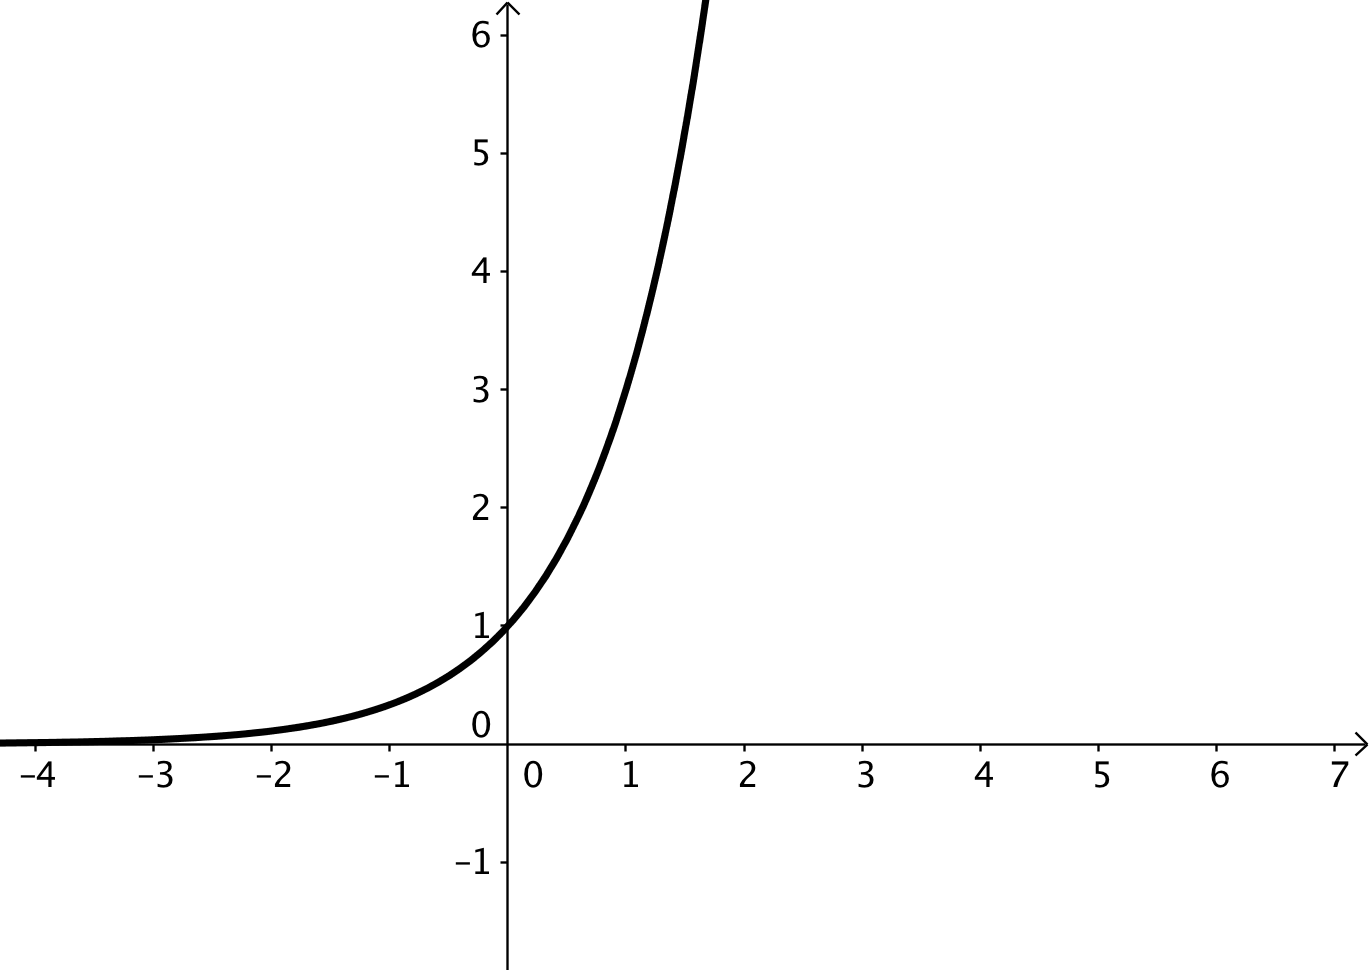
\includegraphics{exp1}} &   \scalebox{0.4}{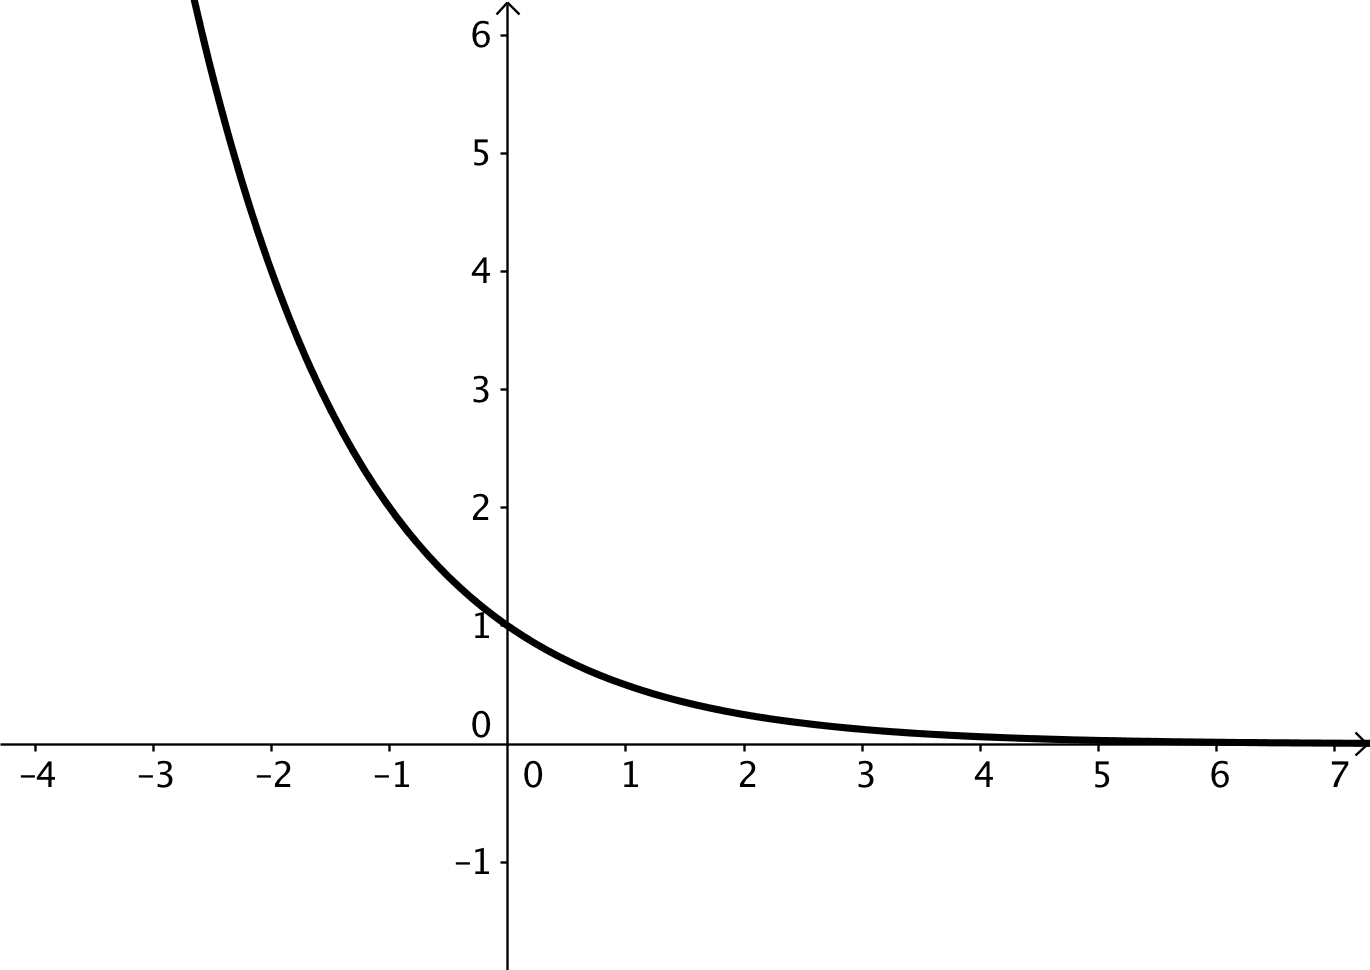
\includegraphics{exp2}} \\
always increasing & always decreasing \\
one-to-one & one-to-one \\
has an asymptote of $y=0$  & has an asymptote of $y=0$ \\
$y$-intercept is $(0,1)$, no $x$-intercept & $y$-intercept is $(0,1)$,  no $x$-intercept  \\
\end{tabular} 
\end{center}

\scalebox{0.9}{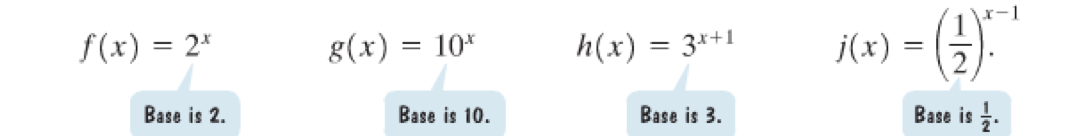
\includegraphics{expex}} 



\begin{enumerate}

\item Is $f(x)=1^x$ an exponential function?\\[.5in]



\item Is $f(x)=(-4)^x$ an exponential function?\\


\newpage
\item Graph $f(x)=3^{x-2}+4.$\\
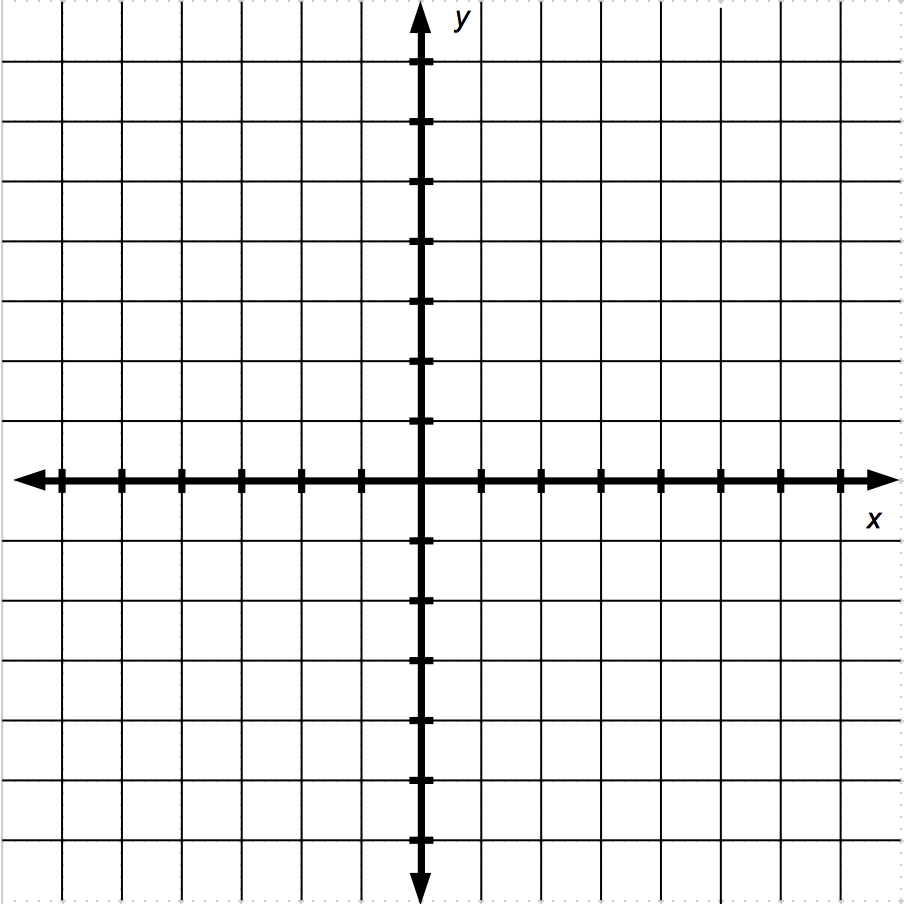
\includegraphics[scale=.5]{bigaxes}

\item Determine the domain and range of $y=5^{x-3}+4$.  \\[1in]





\subsection{Exponential Function Base $e$} 
Just like the number $\pi \approx 3.14159$ is important to the study
of circles and angle measures, the number $e \approx 2.71828$ is
important to problems involving exponential exponential functions (and
their inverses).

Where does the number $e$ come from? Consider the expression $$\Bigg(1+\frac{1}{n}\Bigg)^n$$
If you plug in larger and larger values for $n$, this expression gets closer and closer to $e$.  Try it out!\\
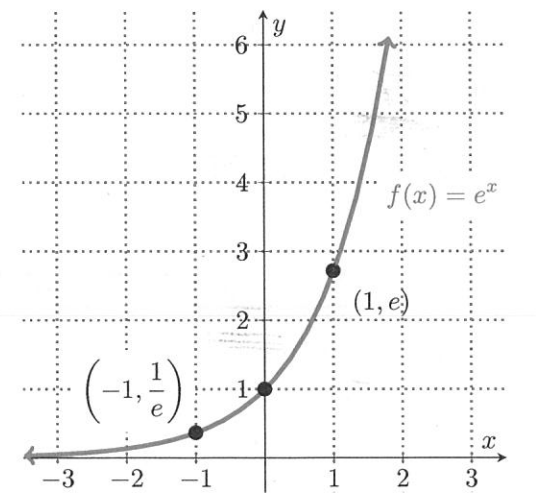
\includegraphics[scale=.8]{e}





\subsection{Compound Interest} ~

\hspace{-.3in} \begin{tabular}{ | l  |} \hline 
\noindent \underline{Compound Interest Formula (Annually, Monthly, Quarterly, Daily, Etc.)}  
$A= P \left( 1+ \dfrac{r}{n} \right)^{nt}$ \\ 
In this formula, $P$ is the principal, $r$ is the annual interest rate in decimal form, $n$ is\\ the number of interest periods per year, $t$ is the number of years $P$ is invested, and $A$ is the\\ amount after $t$ years. \\ \hline
\end{tabular} 

\item Suppose \$ 2000 is invested at a rate of $3 \%$ compounded monthly. Find the \emph{principal after 18 months}. (Round your answer to the nearest cent.) \vfill


 \hspace{-.3in} \begin{tabular}{| l |} \hline
\underline{Continuously compounded interest formula} $A = Pe^{rt}$ \\
In this formula, $P$ is the principal, $r$ is the annual interest rate in decimal form, 
$t$ is the\\ number of years $P$ is invested, and
$A$ is the amount after $t$ years.   \\ \hline
\end{tabular}


\item If \$1500 is deposited in a savings account that pays interest at a rate of .1\% compounded continuously, find the balance after 7 years. \\[1in]


\newpage

\subsection{Exponential Functions in Applications} 
Increasing and decreasing exponential functions can be used in a
variety of real world applications.  For example:
\begin{itemize}
\item Population growth can often be modeled by an exponential function.
\item The growth of an investment under compound interest increases exponentially.
\item The mass of a radioactive substance decreases exponentially with time.
\end{itemize}

\noindent A substance that undergoes radioactive decay is said to be radioactive.  The \textbf{half-life} of a radioactive substance is the amount of time it takes for one-half of the original amount of the substance to change into something else.

\item The half-life of radium 226 is 1620 years.  In a sample originally having 1 gram of radium 226, the amount $A(t)$ in grams of radium 226 present after $t$ years is given by $\displaystyle A(t)=(\frac{1}{2})^{t/1620}$ where $t$ is the time in years after the start of the experiment.  How much radium will be present after 3240 years? 
\vfill


\end{enumerate}

\noindent \textbf{Student Learning Outcomes Check}

\begin{enumerate}
\item Can you recognize an exponential function graphically and algebraically?
\item Can you evaluate the exponential function base $e$?
\item Are you able to use exponential functions in compound interest and growth/decay problems?

\end{enumerate}

\noindent \textbf{If any of your answers were no, please ask about these topics in class.}

